% Written by appendix_genetic/make_tikz.py. Do not edit by hand.
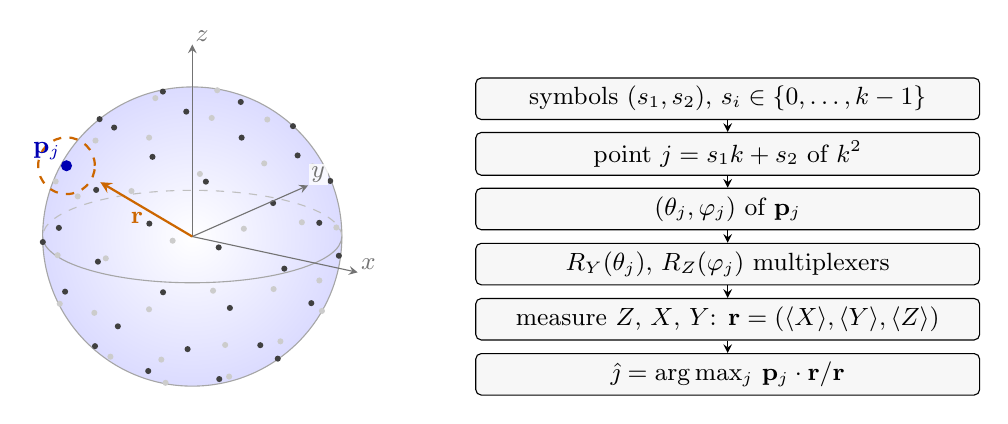
\begin{tikzpicture}[>=stealth, font=\small]
\begin{scope}
\shade[inner color=white, outer color=blue!14] (0,0) circle (1.9);
\draw[gray!70] (0,0) circle (1.9);
\draw[gray!50, dashed] (1.9,0) arc (0:180:1.9 and 0.587);
\draw[gray!70] (-1.9,0) arc (180:360:1.9 and 0.587);
\fill[fill=black!75] (-0.076,1.586) circle (1.1pt);
\fill[fill=black!75] (-0.373,1.841) circle (1.1pt);
\fill[fill=black!75] (0.616,1.709) circle (1.1pt);
\fill[fill=black!75] (-0.992,1.384) circle (1.1pt);
\fill[fill=black!20] (0.317,1.858) circle (1.1pt);
\fill[fill=black!75] (0.627,1.256) circle (1.1pt);
\fill[fill=black!75] (-1.177,1.491) circle (1.1pt);
\fill[fill=black!75] (1.279,1.402) circle (1.1pt);
\fill[fill=black!75] (-0.505,1.012) circle (1.1pt);
\fill[fill=black!20] (-0.469,1.758) circle (1.1pt);
\fill[fill=black!75] (1.338,1.030) circle (1.1pt);
\fill[fill=black!20] (0.953,1.486) circle (1.1pt);
\fill[fill=black!75] (0.173,0.697) circle (1.1pt);
\fill[fill=black!20] (-1.229,1.219) circle (1.1pt);
\fill[fill=black!75] (1.752,0.706) circle (1.1pt);
\fill[fill=black!75] (-1.220,0.592) circle (1.1pt);
\fill[fill=black!20] (0.247,1.506) circle (1.1pt);
\fill[fill=black!75] (1.027,0.425) circle (1.1pt);
\fill[fill=black!20] (-1.735,0.700) circle (1.1pt);
\fill[fill=black!20] (1.527,0.891) circle (1.1pt);
\fill[fill=black!75] (-0.545,0.164) circle (1.1pt);
\fill[fill=black!20] (-0.548,1.256) circle (1.1pt);
\fill[fill=black!75] (1.613,0.174) circle (1.1pt);
\fill[fill=black!75] (-1.694,0.110) circle (1.1pt);
\fill[fill=black!20] (0.914,0.929) circle (1.1pt);
\fill[fill=black!75] (0.336,-0.138) circle (1.1pt);
\fill[fill=black!20] (-1.455,0.510) circle (1.1pt);
\fill[fill=black!20] (1.830,0.115) circle (1.1pt);
\fill[fill=black!75] (-1.198,-0.319) circle (1.1pt);
\fill[fill=black!20] (0.097,0.795) circle (1.1pt);
\fill[fill=black!75] (1.169,-0.408) circle (1.1pt);
\fill[fill=black!75] (-1.898,-0.070) circle (1.1pt);
\fill[fill=black!20] (1.392,0.181) circle (1.1pt);
\fill[fill=black!75] (-0.371,-0.708) circle (1.1pt);
\fill[fill=black!20] (-0.772,0.578) circle (1.1pt);
\fill[fill=black!75] (1.862,-0.244) circle (1.1pt);
\fill[fill=black!75] (-1.615,-0.700) circle (1.1pt);
\fill[fill=black!20] (0.655,0.099) circle (1.1pt);
\fill[fill=black!75] (0.478,-0.907) circle (1.1pt);
\fill[fill=black!20] (-1.710,-0.237) circle (1.1pt);
\fill[fill=black!20] (1.614,-0.558) circle (1.1pt);
\fill[fill=black!75] (-0.945,-1.140) circle (1.1pt);
\fill[fill=black!20] (-0.249,-0.053) circle (1.1pt);
\fill[fill=black!75] (1.512,-0.846) circle (1.1pt);
\fill[fill=black!20] (-1.683,-0.854) circle (1.1pt);
\fill[fill=black!20] (1.033,-0.667) circle (1.1pt);
\fill[fill=black!75] (-0.059,-1.430) circle (1.1pt);
\fill[fill=black!20] (-1.098,-0.277) circle (1.1pt);
\fill[fill=black!20] (1.647,-0.945) circle (1.1pt);
\fill[fill=black!75] (-1.235,-1.392) circle (1.1pt);
\fill[fill=black!20] (0.264,-0.688) circle (1.1pt);
\fill[fill=black!75] (0.864,-1.380) circle (1.1pt);
\fill[fill=black!20] (-1.244,-0.969) circle (1.1pt);
\fill[fill=black!20] (1.120,-1.331) circle (1.1pt);
\fill[fill=black!75] (-0.559,-1.708) circle (1.1pt);
\fill[fill=black!20] (-0.549,-0.924) circle (1.1pt);
\fill[fill=black!75] (1.086,-1.551) circle (1.1pt);
\fill[fill=black!20] (-1.039,-1.526) circle (1.1pt);
\fill[fill=black!20] (0.418,-1.377) circle (1.1pt);
\fill[fill=black!75] (0.343,-1.810) circle (1.1pt);
\fill[fill=black!20] (-0.393,-1.563) circle (1.1pt);
\fill[fill=black!20] (0.468,-1.779) circle (1.1pt);
\fill[fill=black!20] (-0.339,-1.858) circle (1.1pt);
\draw[->, black!55] (0,0) -- (0.000,2.439) node[anchor=south west, inner sep=1pt, fill=white, fill opacity=0.8, text opacity=1] {$z$};
\draw[->, black!55] (0,0) -- (2.101,-0.455) node[anchor=south west, inner sep=1pt, fill=white, fill opacity=0.8, text opacity=1] {$x$};
\draw[->, black!55] (0,0) -- (1.471,0.649) node[anchor=south west, inner sep=1pt, fill=white, fill opacity=0.8, text opacity=1] {$y$};
\draw[orange!80!black, thick, dashed] (-1.597,0.899) circle (0.36);
\draw[->, thick, orange!80!black] (0,0) -- (-1.167,0.690);
\node[orange!80!black, anchor=north east, inner sep=1pt] at (-0.584,0.345) {$\mathbf{r}$};
\fill[blue!70!black] (-1.597,0.899) circle (2pt);
\node[blue!70!black, anchor=south east, inner sep=2pt] at (-1.597,0.899) {$\mathbf{p}_j$};
\end{scope}
\node[draw, rounded corners=2pt, fill=gray!6, minimum width=6.4cm, inner sep=3pt] (s0) at (6.800000000000001,1.75) {symbols $(s_1, s_2)$, $s_i \in \{0,\dots,k-1\}$};
\node[draw, rounded corners=2pt, fill=gray!6, minimum width=6.4cm, inner sep=3pt] (s1) at (6.800000000000001,1.05) {point $j = s_1 k + s_2$ of $k^2$};
\draw[->] (s0) -- (s1);
\node[draw, rounded corners=2pt, fill=gray!6, minimum width=6.4cm, inner sep=3pt] (s2) at (6.800000000000001,0.35) {$(\theta_j, \varphi_j)$ of $\mathbf{p}_j$};
\draw[->] (s1) -- (s2);
\node[draw, rounded corners=2pt, fill=gray!6, minimum width=6.4cm, inner sep=3pt] (s3) at (6.800000000000001,-0.35) {$R_Y(\theta_j)$, $R_Z(\varphi_j)$ multiplexers};
\draw[->] (s2) -- (s3);
\node[draw, rounded corners=2pt, fill=gray!6, minimum width=6.4cm, inner sep=3pt] (s4) at (6.800000000000001,-1.05) {measure $Z$, $X$, $Y$: $\mathbf{r} = (\langle X\rangle, \langle Y\rangle, \langle Z\rangle)$};
\draw[->] (s3) -- (s4);
\node[draw, rounded corners=2pt, fill=gray!6, minimum width=6.4cm, inner sep=3pt] (s5) at (6.800000000000001,-1.75) {$\hat{\jmath} = \arg\max_j \, \mathbf{p}_j \cdot \mathbf{r} / \lVert \mathbf{r} \rVert$};
\draw[->] (s4) -- (s5);
\end{tikzpicture}
